\section{Introduction}
Today the need for stable webapplications is vital for companys and startups. Established businesses need to be
available for their customers and users all the time. For Startups the availability of their services can be the difference
between failure and success. Webapplications and services needs to change and scale over time. Sometimes it is the need
to open up your service for more customers, like Runtastic, a small company from Linz/austria. They developed
a fitness application whose userbase was growing in a short periode of time. Somtimes the customerbase demands a 24/7
availability, for example the sales platform Amazon or the social network Facebook. When Facebook took an outage on September 28 2015,
this incident got a huge ammount of interest from local, national and international media (\url{http://www.bbc.com/news/world-us-canada-34383655}.

Downtime is costly. In the best case it only costs money, in the worst case
it can be the failure of your business or startup. All the mentioned services and events have one thing in common. To provide this kind of zero
downtime and continuous change in your webapplication you need a reliable and stable automatisation for your services. Development operations are
right now one of the major topics in webdevelopment. If used properly, DevOps can provide this kind of zero downtime and progress in an application
(\cite{humble2010continuous} \cite{duvall2007continuous}). To do so DevOps can use a variaty of techniques and methods to continuously
integrate, automatic test and deploy an applications (\cite{meyer2014continuous}).
Continuous Integration and development is based on the method of agile software development and extrem programming
(\cite{lindstrom2004extreme}). There is a reliable base of knowledge and literature for Continous Integration today
(\cite{schaefer2013continuous}), (\cite{fowler2006continuous}) (\cite{fowler2012continuous}).

However, some of the newer methods, for example MEAN stack or NodeJS are not yet fully covered.
The Question i will research in this thesis is, how can a modern webapplication automatized and deployed to continously integrate features and
changes. It is my goal to show how to establish a modern development operation cycle for webapplications using Node.js and the MEAN stack.
I will citeing the standard literature and methods for continuous integration and deployment and show how to build them in a safe and stable
way with Node.js and other Parts of the MEAN stack.
For this i will study the literatur that is available for continuous integration and autmatization to build a similar system with NodeJs.
To do so i will describe how to automatize builds and tests and how to use containerization to simplify the process. Based on the
implementation cycle of the neolexon webapplication, i will provide data to prove that this setup is capable of continous integration and deployment
ant that it runs in a stable and reliable.

\newpage

\section{Introduction to Agile Development and the Role of Development Operations in Modern Web Applications}
\label{section:Introduction to Agile Development and the Role of Development Operations in Modern Web Applications}

% start here
\subsection{Engineering Software}
Webdevelopment has its roots in general software engineering and uses most of the models, tools and methodologies that are
common in the field of software development. At the beginning of software development this new field starts with methodologies
and practices that a used, tested and accepted in other engineering subjects like civil engineering or architecture. In civil engineering
a project uses a design phase, which usually provides a detailed plan and, and a construction phase to build exactly after the specified
plan that where invented in the design phase (\cite{lindstrom2004extreme}). Usually, in civil engineering, the construction phase
needs the majority of time and money from the ressources for a given project. In his essay (\cite{fowler2001new}) Martin Fowler writes
that only 10 percent of the available ressources in civil engineering are used for designing and planing a project.
He concludes that using these engineering methodologys have brought software development into trouble, because they seperate design and
construction. To to so means to handle a project like a bridge or building.

A very detailed plan is made, and after a careful mathematical analysis it is descided to put this plan into practice. To construct,
another department or team will provide the actuall construction the bridge.
This seperation makes it possible to use people as ressources in construction, whereafter the design takes place in a more
intellecutal environment. The construction ressources in general dont need to understand the whole design and can concentrate on their
knowledge about constructing. In all this lies a predictability. The trouble for software development with seperation of design and
construction is that the whole process of programming is desiging in the first place. \cite{opac-b1105529} stats that only 15 percent of
a software project is code. This stands in contrast to the building example from civil engineering.

\cite{reeves1992software} therefore suggests that the code of a software project should be used as the design document and that the compilation of the
code should be seen as the main construction phase. For \cite{fowler2001new} the conclusion to Reeves suggestion is the following:
\begin{itemize}
  \item In software: construction is so cheap as to be free
  \item In software all the effort is design, and thus requires creative and talented people
  \item Creative processes are not easily planned, and so predictability may well be an impossible target.
  \item We should be very wary of the traditional engineering metaphor for building software. It's a different kind of activity and requires a different process
\end{itemize} \cite{fowler2001new}

\newpage

\subsection{The Agile Software Manifesto}
Traditional engineering metaphores and separation of design and construction are good for a predictable project where the outcome is clear in
detail to the customer. There is no such thing as mathematical analysis for software design plans and this means that there will be a very
limited predictability because of all the changes in software development (technical or customer based). To show this in practical detail consider the following
application. This application should provide information for speach therapists in a simple and understandable dashboard in which the user (therapist) gets
an overview. The descision was made that the dashboard should hold only the list of patients and wordlists (figure 1).

\begin{figure}[h!]
  \centering
      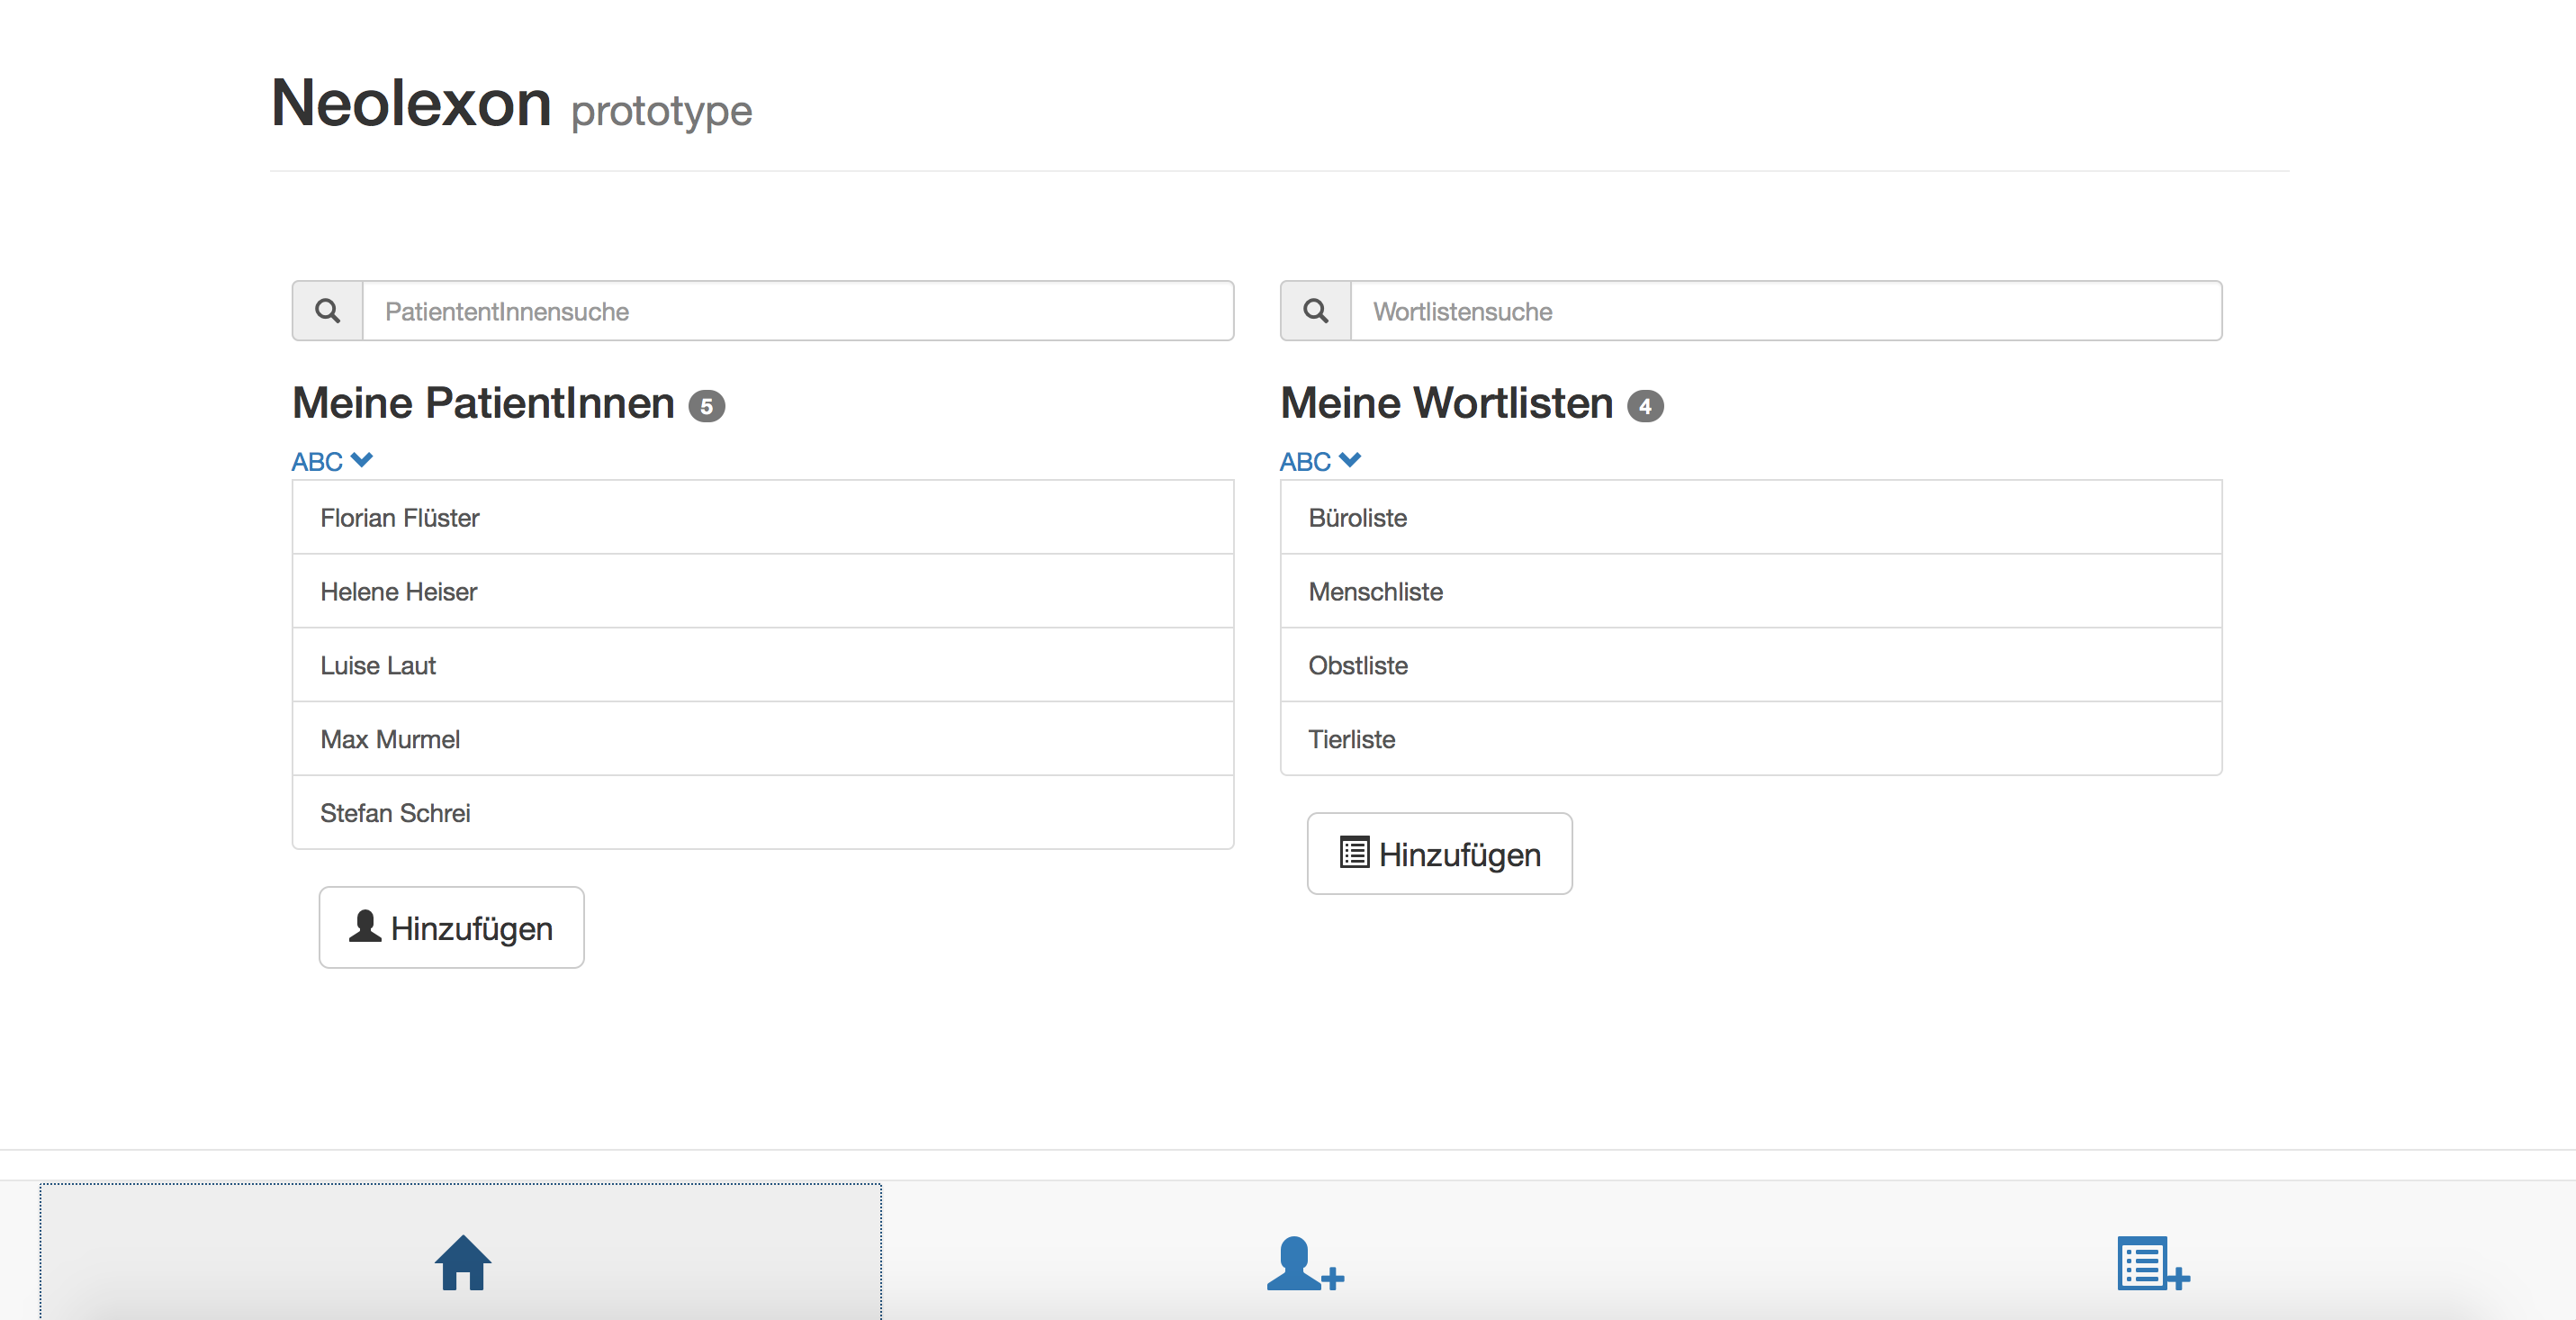
\includegraphics[width=0.8\textwidth]{images/patientsandlists.png}
  \caption{first plan of therapiest dashboard}
\end{figure}

After the dashboard was created and the feedback of several therapists arrived the descision was made that the dashboard dont need to hold the lists
of words, because all lists where individual for the curent patient. This was a total different idea for the wordlists and not in the plan at the beginning.
after this descision the dashboard was not a dashboard anymore, but was left with only the patientlist alone. So the development team came up with another
idea of the dashboard (figure 2)

\begin{figure}[h!]
  \centering
  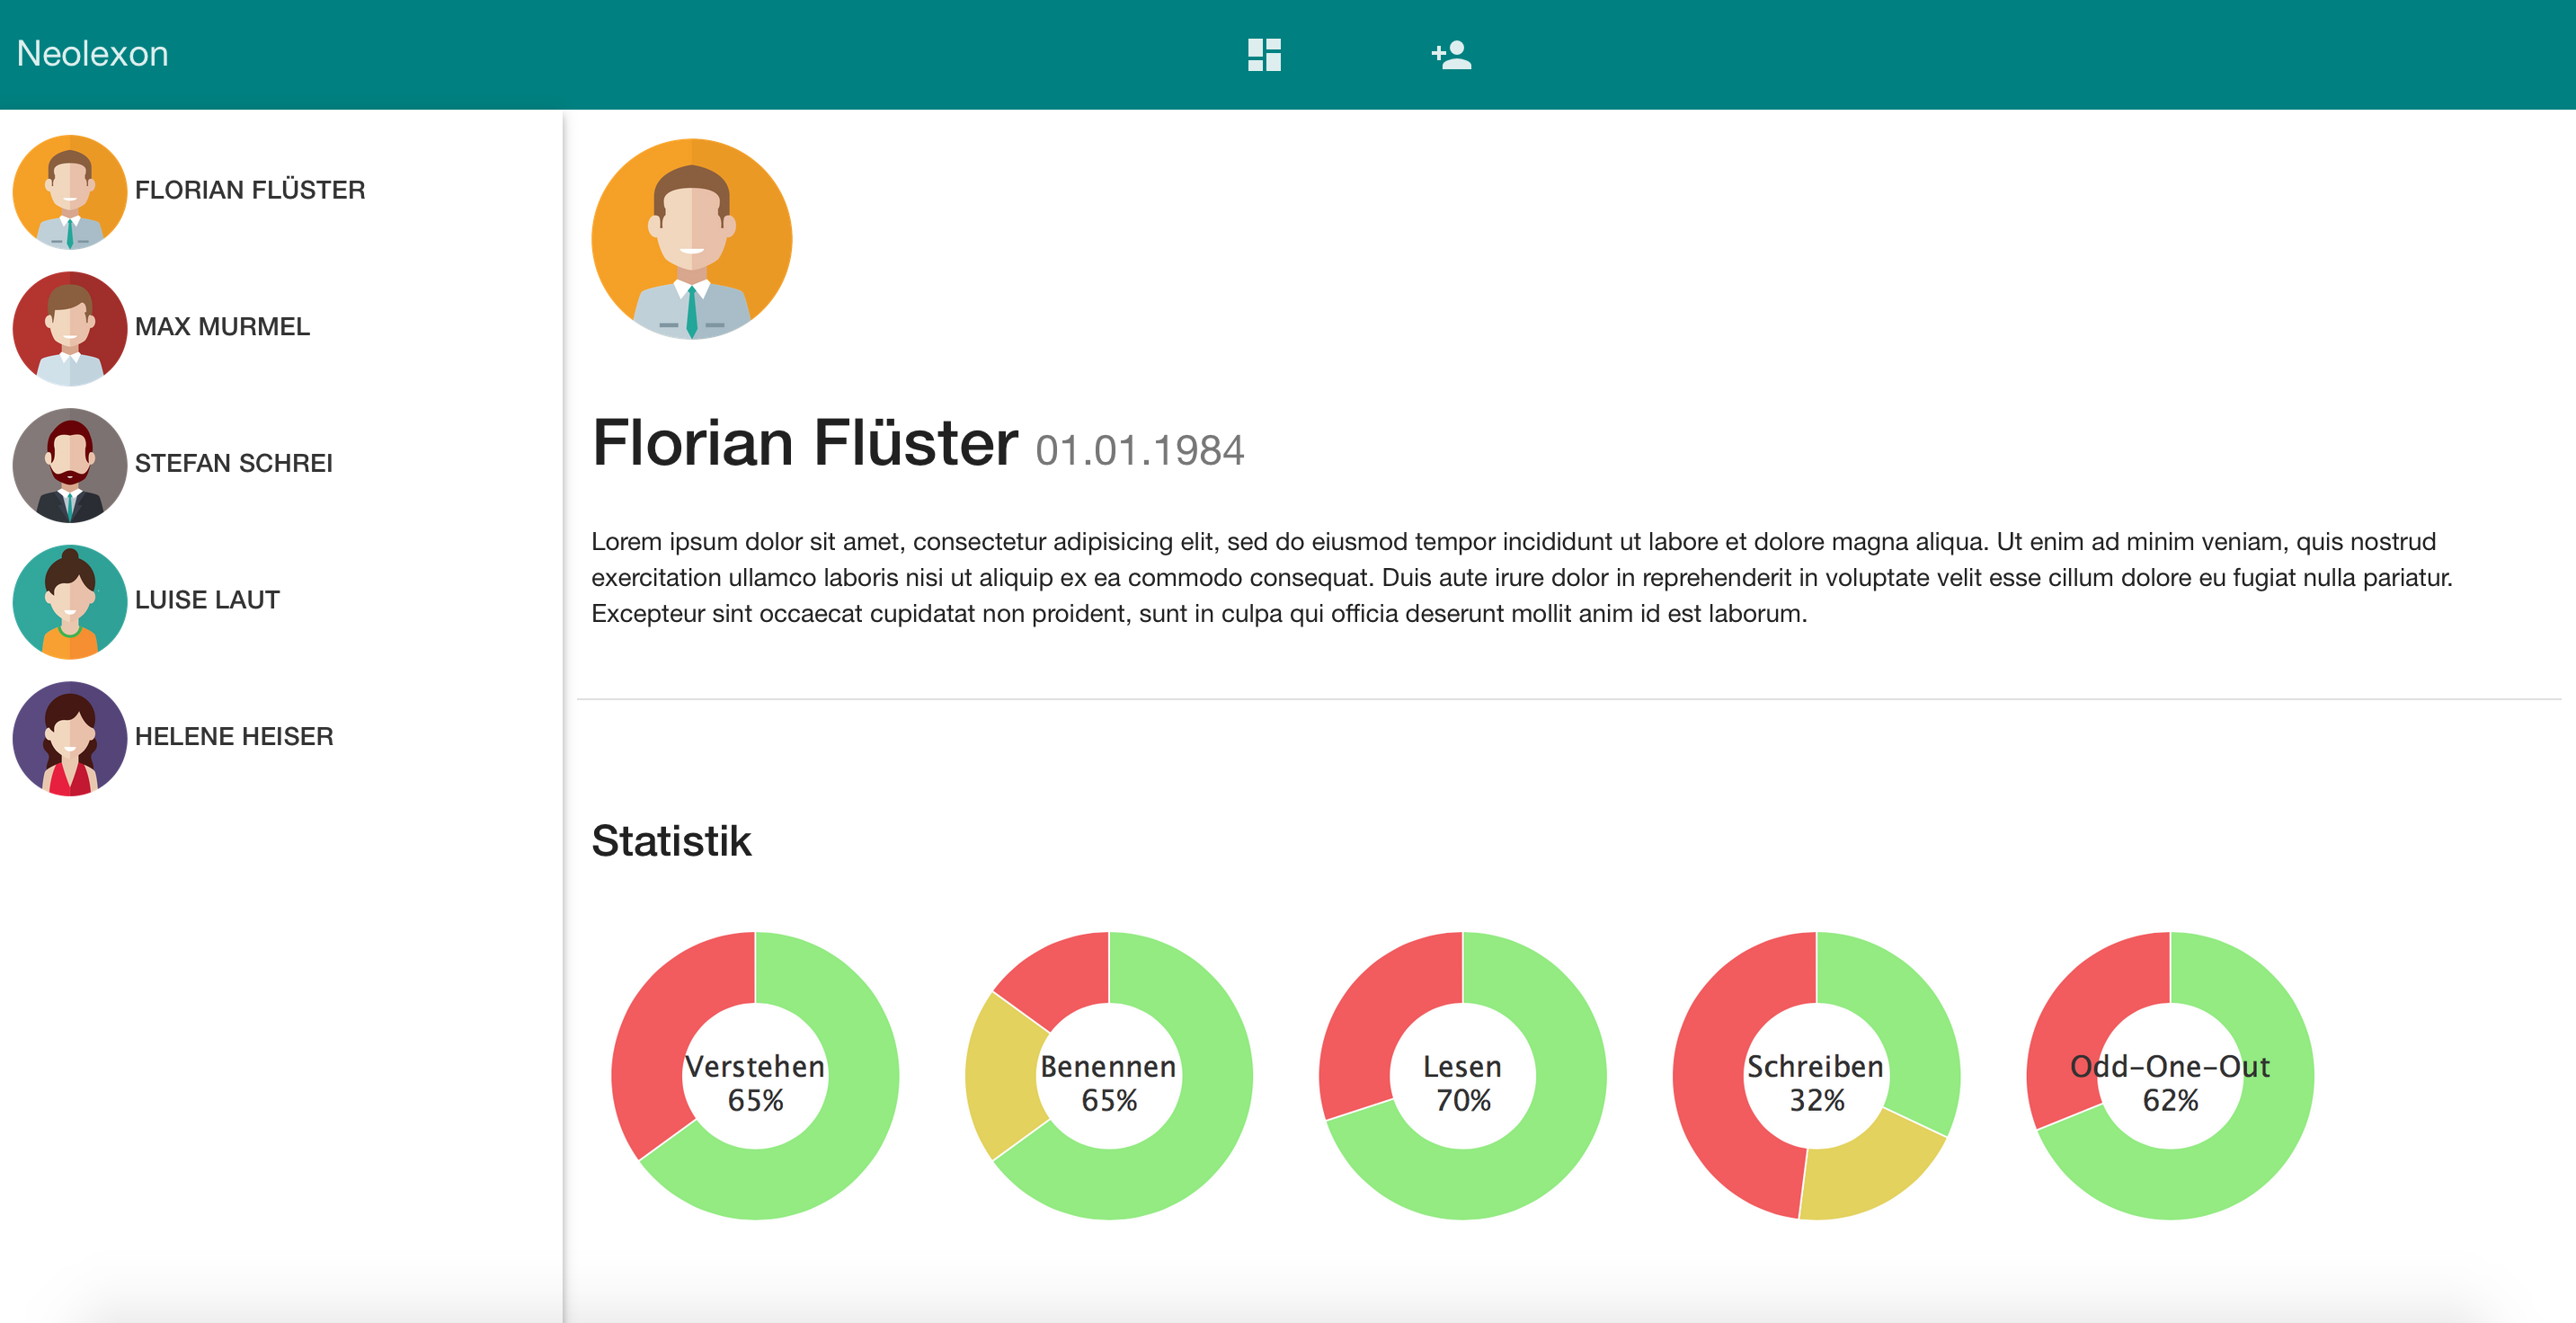
\includegraphics[width=0.8\textwidth]{images/sidenav.png}
  \caption{final dashboard}
\end{figure}

\newpage

As you can see the two ideas differs in layout and idea. According to the initial plan the wordlists should be there. Now you have a sidenavigation
with patients and the statistics for each of them are not bound to the wordlist but are shown in the dashboard. This transformation would have been very
complicated to achieve with traditional engineering methaphore, because the klients only have had seen it at the end of the process. To rebuild a heavily
connected part of a webapplication after the application is finished is very hard to do. This changes toke place in only 2 weeks, from plan to final idea.
So another approache for software development is needed to take difficulties like the described into account.

To conquer this problem, 17 developers (Kent Beck, Mike Beedle, Arie van Bennekum, Alistair Cockburn, Ward Cunningham, Martin Fowler, James Grenning,
Jim Highsmith, Andrew Hunt, Ron Jeffries, Jon Kern, Brian Marick, Robert C. Martin, Steve Mellor, Ken Schwaber, Jeff Sutherland, Dave Thomas)
invented an idea of how to handle a softwareproject. On the 13. of february 2001 they created \textbf{\textit{a Manifesto for Agile Software Development}}.
The Manifesto itself is not a static rule, it is a guideline which can be followed. To make things practicable the Manifesto contains 12 principles about
agile developement.

\begin{itemize}
  \item Our highest priority is to satisfy the customer through early and continuous delivery of valuable software.
  \item Welcome changing requirements, even late in development. Agile processes harness change for the customer's competitive advantage.
  \item Deliver working software frequently, from a couple of weeks to a couple of months, with a preference to the shorter timescale.
  \item Business people and developers work together daily throughout the project.
  \item Build projects around motivated individuals. Give them the environment and support they need, and trust them to get the job done.
  \item The most efficient and effective method of conveying information to and within a development team is face-to-face conversation.
  \item Working software is the primary measure of progress.
  \item Agile processes promote sustainable development. The sponsors, developers and users should be able to maintain a constant pace indefinitely.
  \item Continuous attention to technical excellence and good design enhances agility.
  \item Simplicity—the art of maximizing the amount of work not done—is essential.
  \item The best architectures, requirements and designs emerge from self-organizing teams.
  \item At regular intervals, the team reflects on how to become more effective, then tunes and adjusts its behavior accordingly.
\end{itemize} \cite{fowler2001agile}

\begin{figure}[h!]
  \centering
  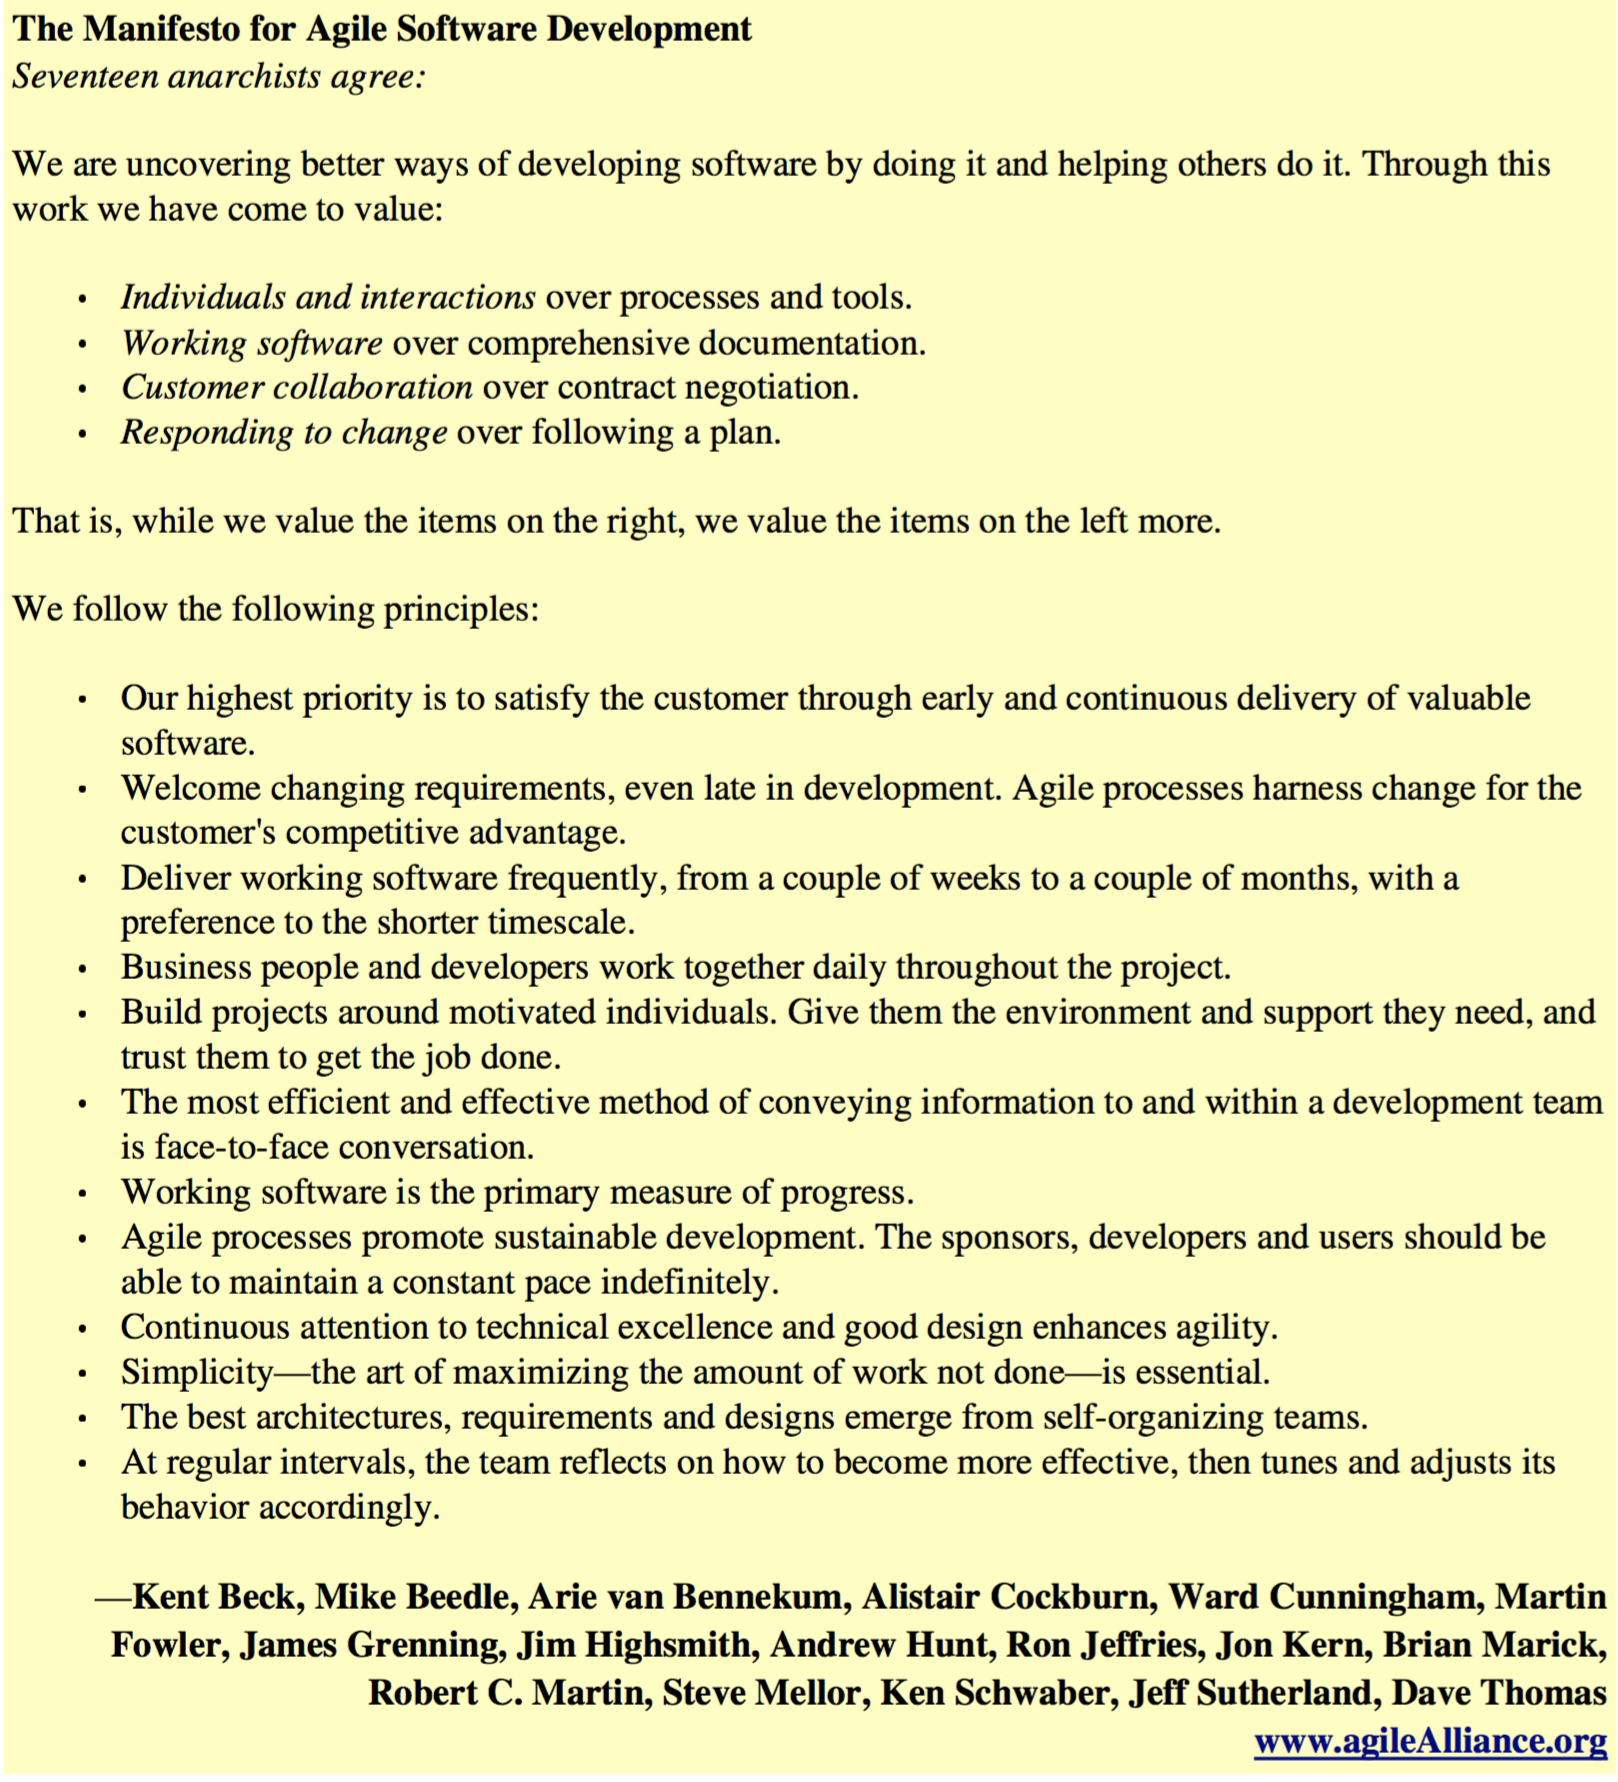
\includegraphics[width=0.8\textwidth]{images/manifesto.png}
  \caption{the agile manifesto}
\end{figure}

% eingehen auf einzelne principles und herleitung zu continuous integration mit sprung zum zweiten kapitel
Based on the manifesto principles it is more realistic to build software. If you stay with the therapist dashboard example the agile approach makes more
sense, compared to a solid plan that starts at the beginning and did not change during the process, because most sofware change in the course of
development. Since many of the principles contain non technical ideas, like a cicle of team reflection, motivating team members or the art of simpicity,
there are solid ideas about how to treat the software and shipping process.

\subsection{Continous integration and delivery}
Right at the start of the manifesto the need for continuous delivery and integration is set as a high priority in development to satisfy the customer.
Satisfing customer needs is one good thing about this approach. Another reason to continuosly integrate software is about the change and the mantainability.
If an application or software changes fast in the development process it is a good idea to ensure that your software is working at every point,
even if the development team or single members change code or adding new features. It is possible to guarantee this in the beginning of a software project,
but when the software grows more complicated and complex it may be impossible to do.

In his book \textbf{\textit{Test-Driven Development by Example}} Kent Beck (\cite{beck2003test}) explains that writing automated tests before the actual
code can be a good service to an applications. As a developer starts to add features and introduce changes into an application that is already
used, automated testing should be a standard. Tests will make sure that problems with existing code or features will be visible after a developer
changes existing parts in the software. That means that the developer did not need to go through all parts of the application manually after some changes
to ensure that everything is still working. To do so is timeconsuming and inefficient, because it is still likley to oversee functionalities in the code
:x
that will be effected by different changes that are made afterwards. It also leads to thought through programming decisions. "The driven in test-dri­ven
development focuses on how TDD leads analy­sis, design, and programming decisions" (\cite{janzen2005test}) which will be of help if the software application
grows larger.


\newpage

\section{The Foundations of Continuous Integration and Automatization in Development Operations}
\label{section:The Foundations of Continuous Integration and Automatization in Development Operations}

% start here

\newpage

\section{Development and Deployment with MEAN}
\label{section:Development and Deployment with MEAN}

% start here

\newpage

\section{Test Driven Development with MEAN}
\label{section:Test Driven Development with MEAN}

% start here

\newpage

\section{Containerization and Deployment with Docker}
\label{section:Containerization and Deployment with Docker}

% start here

\newpage

\section{Building Continuous Integrations and Deployment with NodeJS}
\label{section:Building Continuous Integrations and Deployment with NodeJS}

% start here

\newpage





% \begin{figure}[h!]
%   \centering
%       
\includegraphics[width=0.4\textwidth]{images/Perlin-Coherent.png}
%   \caption{Just some example figure}
% \end{figure}



% \subparagraph{subparagraph}
% \footcite{meyer2014continuous}
%
% \begin{itemize}
%   \item Itemlist 1
%   \item Itemlist 2
% \end{itemize} \cite{cranorplatform}
%
% \section{Next Section}
% \label{section:Label}
%
% \textit{Texit Option}
%
% \begin{figure}[h!]
%   \centering
%       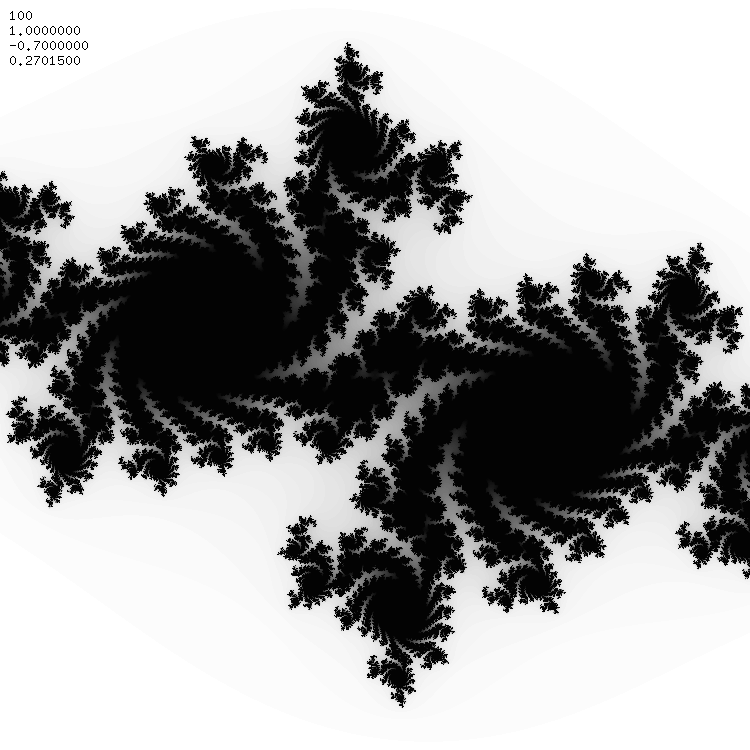
\includegraphics[width=0.2\textwidth]{images/Julia-Fractal.png}
%   \caption{Exampelimage}
% \end{figure}
%
% \subparagraph{Unforgeability}
% \label{subp:subparagraph_name}
%
% Graphic by \url{http://en.wikipedia.org/wiki/Pretty_Good_Privacy#/media/File:PGP_diagram.svg
